Cancer development is a progressive and complex multi-step process within a living system. The uncontrolled growth and cell division properties are general facts which have many hidden implications, both in terms of variables that condition its evolution and, more importantly, its consequences.
\\

Cancer evolution is usually driven by somatic sessions which lead to mutations that confer advantages to the affected cells. The final features of a cancerous cell are said to reveal an accumulation of the alterations acquired along the cell’s life.

These altered cells, as a result of fitting mutations accumulation, eventually populate the environment and overtake its competitors presence (healthy individuals or misfit clones) via clonal expansions. Their fitness plays then an important role on its evolution and, therefore, survival.
\\

Many studies \cite{Rifai2006ProteinUtility}\footnote{In order to avoid over-referencing, the linked document gathers several studies focusing on biomarkers.} focus precisely on biomarkers: measurable specific characteristics which identify a condition in order to find a clear differentiating factor for specific cancer types. These can lead the investigation to identifiable drug targets which to action clinically. Usually the most effective target biomarkers are driver mutations, 
alterations which confer growth advantage to cells which carry them, hence enhancing their positive selection in cancer evolution \cite{Stratton2009TheGenome}.

However, the efficiency of these methods in clinical trials is widely unknown and unpredictable. Drug low-response and patients relapse are common issues in the oncogenesis field, regularly related to the cancer’s heterogeneity. Cancerous cells evolution are highly dependent on patient’s genome and environment \cite{Yates2012EvolutionGenome}. Altogether, they build the niche where cancer differentiation, even within a subtype, is plausible. There is evidence that several individuals diagnosed under the same condition, have different evolution and prognosis \cite{Gao2016LossTherapy}, \cite{Zaretsky2016MutationsMelanoma}, mainly due to a potential assorted property of a cancerous tissue, which eventually leads to relapse due to patient's organism unresponsiveness to treatment.
\\

\subsection{Gene chronological order}
Based on previously discussed heterogeneity, multimodal\footnote{Referring to reaching several distinct outcomes in phenotype and/or genotype terms.} and divergent evolution scenarios are feasible, where dissimilar cancer populations arise. Each cell progeny might accumulate different mutations -- although keeping the core ones--, or exactly the same mutations but in different order.

In terms of causality, another factor which adds complexity is the issue of discerning amongst mutations which happen due to the enhancing effect of another mutation(s) happening (triggered dysregulation), or the acquired ones (somatic), such as radiation, DNA replication mismatches, etc., which in turn cause the first kind.
\\

As a general first approach, cancer types can be identified based on molecular and genetic information, e.g. Breast cancer has 4 genetically different known subtypes: Luminal A, Luminal B, Triple negative/basal-like and HER2-enriched, which accumulate different mutations, and therefore drive to divergent behaviours and prognosis.

However, within the same subtype, populations can also be different in genomics terms and/or behavioural, i.e. different evolution compared to its peers \cite{Melo2013CancerView} \cite{Kent2017OrderEvolution}. Natural selection then acts upon, where the survival of the fittest prevails, and finally tumour development evolves from an individual which would become the original common ancestral clone —which may or may not still be present around afterwards— into a fully diverse cell community. Similarity and heterogeneity degree within the neighbourhood will ultimately rest on the microenvironment\footnote{TME or Tumor MicroEnvironment has been largely studied, and the results have been put together in:\url{https://www.sciencedirect.com/topics/medicine-and-dentistry/tumor-microenvironment}}.
\\

Consequently, not only identical tumours share few gene alterations, but also show different mutation order acquisition. Then, does this chronological order [in which mutations happen] affect the evolution of the disease?

This work bases its hypotheses on mutation chronological order, hence assuming a chronological order in mutation events, cancer evolution can be seen as a diagram of branched events, more or less probable to converge to the same state\footnote{We expect a modelling similar to a phylogenetic tree, in which divergence and evolution from a common ancestor has a tree-like shape. The main definition of a \emph{tree} in graph theory does not allow for cycles or convergence of any kind. Here we refer to phenotypical convergence, i.e. an accumulation of mutations which eventually deliver the same outcome. Genetically, only clones evolving in the same branch would remain genetically equal and/or systemically dysregulated.}, depending on the mutation acquisition synergy effect.
\\

As a consequence, classification, patient stratification or prediction can be done based on the stage’ history trace back analysis. Prognosis can be based on time-point samples \cite{Spencer2006ModelingTumorigenesis} along during the case study, and early action to target the drivers, although delicate to calculate, would suppose a step forward in precision. 
\\

\subsection{Pathway-driven ordering}
A common belief is that a cell needs to acquire certain mutation-driven properties in order to become carcinogenic. Generally, these include a potential capacity of avoiding apoptosis, unlimited replication power, unresponsiveness to (external) signals, angiogenesis and other tissues invasion, among others \cite{Hanahan2011HallmarksGeneration}. The regulation of such biological functions are bound to the cell’s pathway. Many point dysregulation events in these systems are related to cell’s malfunction.
\\

Picking up from the single-gene-mutation modelling above, where we focus on individual genes mutation, we cannot leave out further implications of this case: Gene mutation and consequent defective function has a cascade effect on the pathway it's related to (Figure \ref{fig:gp}). Studies like \cite{Gerstung2011TheTumorigenesis} found up to 70\% pathway alteration frequency in all analysed samples. Therefore, selective pressure ultimately has an impact at pathway level, as gene alteration order eventually dysregulates interconnected pathways.
\\

\begin{figure}
    \centering
    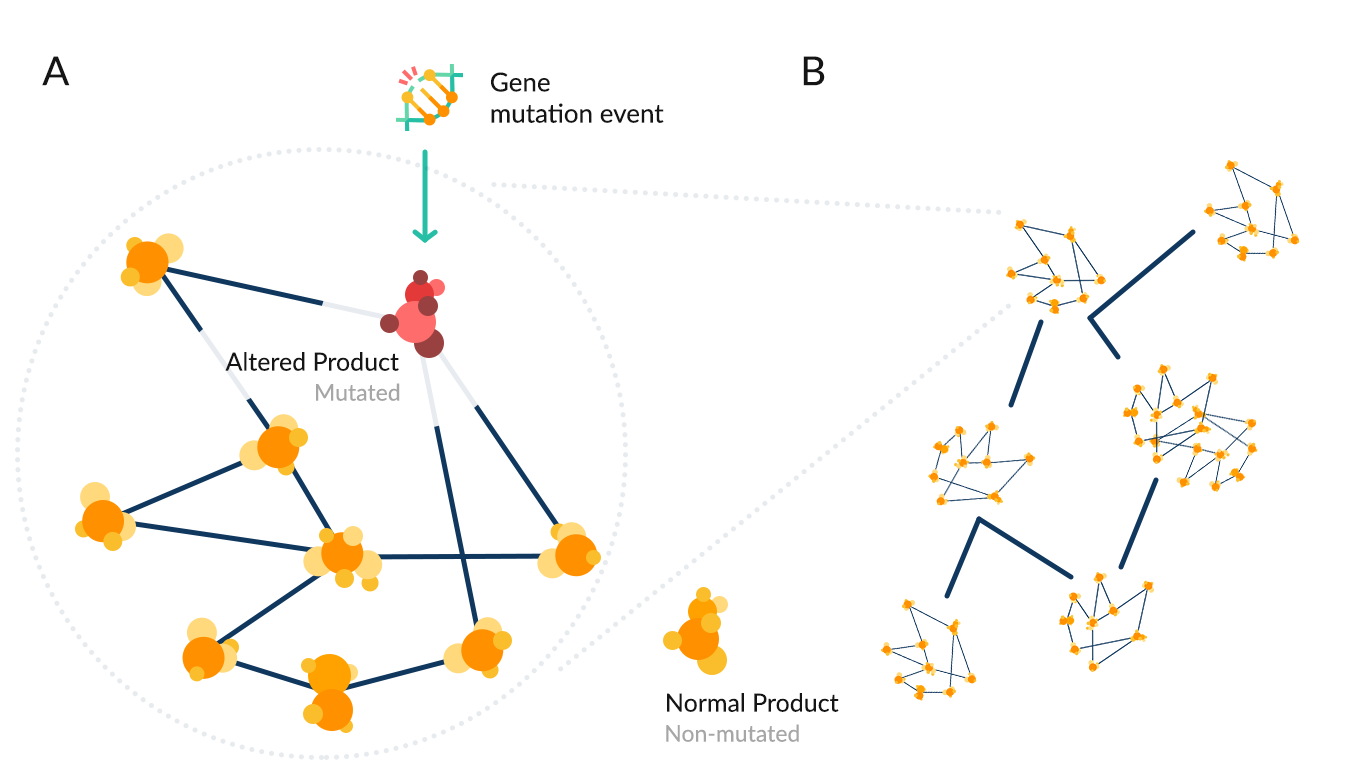
\includegraphics[width=\linewidth]{images/GP.png}
    \caption{Schema relating gene- and pathway-based order approaches. (A) displays the known fact of a mutational event disrupting the regular behaviour of all the items interacting with its altered product. (B) shows how the previous dysregulation, which acts at pathway level, has triggers deeper consequences across all related pathways.}
    \label{fig:gp}
\end{figure}

Nevertheless, and assuming cell signalling universality, pathway dysregulation might differ from one patient to another \cite{Ulitsky2010DEGAS:Diseases}. In fact, same cancer type diagnosed in different patients can result in vast heterogeneity of cases due to different dysregulation events trajectories (within same or different pathways) \cite{Khakabimamaghani2019UncoveringDysregulation}.
\\

A pathway-driven approach can be advantageous in that we can combine sporadic mutations a simple single event, which allows better comparison of functional consequences, in the same way profile-driven has advantages over sequence-sequence comparison \cite{Cheng2012AGliomagenesis}.

Is then this temporal order responsible for heterogeneous yet highly-similar pathways dysregulation among patients under the same diagnosis?
Previous background of individuals, such as environment exposure (nutrition, smoking, ambient factors, etc.) \cite{Jung2007EnvironmentalGenome} already sets different starting points from which a condition can be developed, i.e. the genetic scenario influences an individual’s evolution, both as a healthy organism or as a diseased one. Thus sequential component not only can be influential, but more prominent in clinical followup.

\subsection{Inheritance implications in the picture}

Notwithstanding, aside of somatic mutations, the genetic luggage we carry is also influential in evolution and tracking. Inherited mutations cause 5-10\% of family cancer syndromes, making certain individuals more prone to develop a condition than others.
\\

Following gene inheritance basics, if a a person inherits a mutation in a DNA copy of a tumour suppressor gene, would only need the other copy to mutate for the gene to malfunction, hence having a higher risk of triggering the oncogenesis process. In terms of gene and/or pathway ordering this has an immediate implication: Events occurring in an exceptional\footnote{DNA/Gene alterations can already be considered exceptional. The abnormality we mention is related to \emph{time expectancy}, i.e. we expect A happening before B, but B occurs before A.} chronological order interfere with assorting procedures proposed above. A simple example would be discerning chronological placement errors for a mutation which usually belongs to late stages of cancer but it has been inherited from a parent, hence, sequentially it has happened in the earliest stage. Its magnitude, of course, is linked to the event real effect within the whole system.

We then ask: Do inherited mutations have an impact on the order genes suffer mutations? Is it larger than somatic mutations?
\\

At first sight we can hypothesise that inheritance acts as a barrier for tracing, since heritage is commonly missing in the analysis. Any model based on chronology which experiences reordering in its items will fail at delivering a solid display of the events. However, prediction can only be made on patient’s evolution and, although historic might help foresee response, problems and evolution, it sets challenges to collect an accurate model.